\documentclass[13pt]{article}
\usepackage[utf8]{inputenc}
\usepackage[T2A]{fontenc}
\usepackage[russian]{babel}
\usepackage{amsmath}
\usepackage{amssymb}
\usepackage{setspace}
\usepackage{titlesec}
\usepackage{blindtext}
\usepackage{mathtext}
\usepackage{bm}
\usepackage{esvect}
\usepackage{graphicx}
\usepackage{longtable}
\usepackage{textcomp}
\usepackage{geometry} 
\usepackage{pgfplots}
\usepackage{circuitikz}
\usepackage{indentfirst}
\pgfplotsset{compat=1.9}
\geometry{verbose,a4paper,tmargin=2cm,bmargin=2cm,lmargin=3.0cm,rmargin=1.5cm}
\usepackage[style=numeric]{biblatex}
\addbibresource{sample.bib}
\graphicspath{{images/}}
\DeclareGraphicsExtensions{.pdf,.png,.jpg,.gif}
\pagestyle{plain}
\RequirePackage{caption}
\DeclareCaptionLabelSeparator{defffis}{ - }
\addto\captionsrussian{\renewcommand{\figurename}{Рисунок}}
\DeclareCaptionFormat{1}{2}
\captionsetup{justification=centering,labelsep=defffis}
\usepackage{pgf, tikz}
\usetikzlibrary{arrows,automata,positioning}

\addto\captionsenglish{% Replace "english" with the language you use
  \renewcommand{\contentsname}%
    {Оглавление}%
}
\begin{document}
\begin{titlepage}                                                         
    \newpage                                                                        
    \begin{center}                                                        
    {\bfseries Министерство науки и высшего образования Российской Федерации \\
    НАЦИОНАЛЬНЫЙ ИССЛЕДОВАТЕЛЬСКИЙ ЯДЕРНЫЙ УНИВЕРСИТЕТ <<МИФИ>>}                               
    \vspace{1cm}                                                          
                                                  
    ИНСТИТУТ ИНТЕЛЛЕКТУАЛЬНЫХ КИБЕРНЕТИЧЕСКИХ СИСТЕМ\\
    КАФЕДРА КОМПЬЮТЕРНЫЕ СИСТЕМЫ И ТЕХНОЛОГИИ
    \vspace{6em}                                                          
    \end{center}                                                          
                                                                                        
    \vspace{1.2em}       

                                                                                        
    \begin{center}                                                        
    %\textsc{\textbf{}}                                     
    \Large Пояснительная записка по курсу \linebreak \textbf{<<Схемотехническая база цифровых устройств>>} \linebreak
    на тему: \linebreak
    \textbf{<<Проектирование кэш-памяти>>}
    \end{center}                                                          
    \vspace{20em}                                                                           
    \vbox{%
    \hfill%
    \vbox{%
    \hbox{Студент гр. М19-512 Никитин С.А. \underline{\hspace{3cm}}}
    \hbox{Преподаватель}
    \hbox{Скитев А.А. \underline{\hspace{3cm}}}
    \hbox{Ядыкин И.М.  \underline{\hspace{3cm}}}
    }%
    }                                                          
    \vspace{\fill}                                                    
                                                                                        
    \begin{center}                                                        
    Москва 2020                                                               
    \end{center}                                                          
                                                                                        
    \end{titlepage} 
	\thispagestyle{empty}
	\newpage
	\tableofcontents
	\newpage
	\section*{Введение}\addcontentsline{toc}{section}{Введение}
	Целью работы является изучение основ структурного проектирования вычислительных систем, овладение современными САПР, получение навыков патентного поиска и исследовательской деятельности. Работа разделена на несколько этапов. Согласно техническому заданию, необходимо выполнить следующие задачи:\\
	1. Подготовить обзор кэш-памяти;\\
	2. Разработать алгоритмы проектируемого устройства;\\
	3. Разработать функциональную схему проектируемого устройства;\\
	4. Реализовать составляющие модули на языке HDL;\\
	5. Объединить модули в общую схему;\\
	6. Обеспечить переход между частотными доменами;\\
	7. Обеспечить тестирование разработанной системы памяти.
	\newpage
	\section{Обзор кэш-памяти}
	\subsection{Организация кэш-памяти}
	\textbf{Кэш-память} --- это высокоскоростная память сравнительно небольшого объема, предназначенная для временного хранения информации. Кэш-память располагается на одном из верхних уровней иерархии памяти. Основная цель --- уменьшение среднего времени доступа к оперативной памяти. 
	Кэш-память состоит из устройства памяти и контроллера. Задачей контроллера является управление работой кэш-памяти: загрузка информации из оперативной памяти, а также отправка модифицрованных данных в оперативную память. Общая схема кэш-памяти представлена на рисунке 1.
	\begin{figure}[h!]
		\center{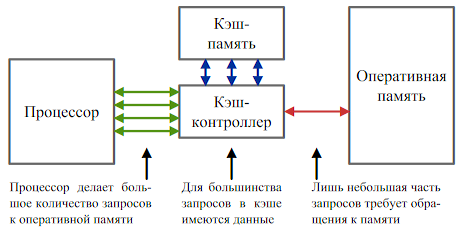
\includegraphics[scale=0.5]{fig1}}
		\caption{Общая схема кэш-памяти}
	\end{figure}
	
	Когда кэш перехватывает запросы к оперативной памяти, кэш-контроллер определяет, есть ли копия передаваемых данных в кэше. Если такая копия есть, то такая ситуация называется \textbf{кэш-попаданием} (hit), иначе - \textbf{кэш-промах} (miss). В случае, если кэш переполнен, работает политика замещения, которая определяет, какие данные должны быть вытеснены. Информация, хранящаяся в кэше, сопровождается метаинформацией (тэгом), который определяет, копией содержания какой ячейки является эта информация.
	
	Различают несколько уровней кэш-памяти процессора:\\
	- L1 Cache (кэш-память первого уровня) --- самая маленькая по объему, но самая быстрая и наиболее важная. Она содержит данные, наиболее часто используемые процессором и работает с минимальными задержками.\\
	- L2 Cache (кэш-память второго уроввня) --- по скорости уступает памяти L1, однако больше по объему. Она предназначена для временного хранения важной информации, вероятность обращения к которой ниже, чем у информации в кэше L1.\\
	- L3 Cache (кэш-память третьего уровня) --- самая большая по объему, но самая медленная, при этом скорость работы значительно выше скорости работы оперативной памяти. Она предназначена для хранения информации, вероятность обращения к которой ниже, чем у информации в L1 и L2. \cite{book:33862}\\
	\subsection{Отображение оперативной памяти на кэш-память}
	\subsubsection{Прямое отображение}
	
	Кэш-память прямого отображения является самой простой реализацией кэш-памяти. В кэш-памяти такого типа заданное слово может храниться только в одном месте. Если его в этом месте нет, то его нет в кэш-памяти вообще. Общая структура памяти с прямым отображением приведена на рисунке 2.
	\begin{figure}[h!]
		\center{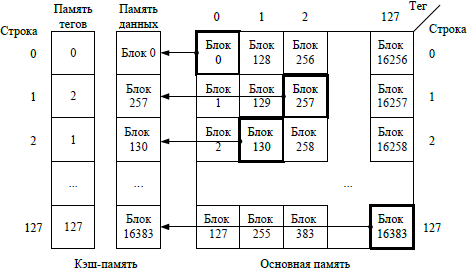
\includegraphics[scale=0.4]{fig2}}
		\caption{Схема памяти с прямым отображением}
	\end{figure}
	
	Как правило, формула отображения - есть остаток от деления адреса строки ОЗУ на количество строк кэш-памяти. При аппаратной реализации для получения адреса строки кэша достаточно убрать старшие биты адреса строки ОЗУ.\\
	Преимущества:\\
	- Простая реализация\\
	- Высокая скорость работы\\
	Недостатки:\\
	- Жесткое закрепление строк кэш-памяти за строками ОЗУ. Если будет обращение к разным блокам ОЗУ, которые отображаются на одни и те же строки кэш-памяти, это приведёт к снижению эффективности из-за постоянной перезаписи строк.
	\subsubsection{Полностью ассоциативное отображение}
	
	При полностью ассоциативном отображении любая ячейка ОЗУ может быть отображена на любую ячейку кэш-памяти. \\
	Преимущество:\\
	1. Возможность одновременно держать в кэш-памяти соседние ячейки ОЗУ.\\
	Недостатки:\\
	1. При большом количестве строк кэш-памяти задача нахождения нужной строки становится достаточно сложной с точки зрения аппаратной реализации.\\
	2. Более медленная, поскольку ассоциативная кэш-память работает последовательно.
	
	Схема полностью ассоциативного отображения приведена на рисунке 3. 
	
	\begin{figure}[h!]
		\center{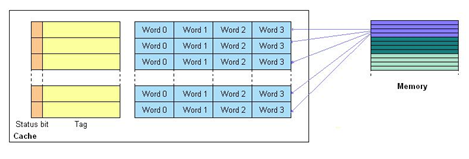
\includegraphics[scale=0.7]{fig3}}
		\caption{Схема памяти с полностью ассоциативным}
	\end{figure}
	\subsubsection{Множественно-ассоциативное отображением}\\
	    Компромиссом между предыдущими двумя методами является метод множественно-ассоциативного отображения. Кэш память разбивается на несколько подмножеств, называемых модулями. Блоки ОЗУ отображаются на модули также, как и при прямом отображении. Отображение строк внутри модуля является ассоциативном. Другими словами в каждом модуле могут присутствовать только строки из определенных блоков ОЗУ, а размещение строк внутри модуля является произвольным. В современных процессорах используется 4 и 8-канальная кэш-память. Увеличение числа ее входов приводит к быстрому увеличению сложности аппаратной реализации той части кэша, которая обеспечивает ассоциативный поиск тегов. Общая схема множественно-ассоциативного отображения приведена на рисунке 4.
	\begin{figure}[h!]
		\center{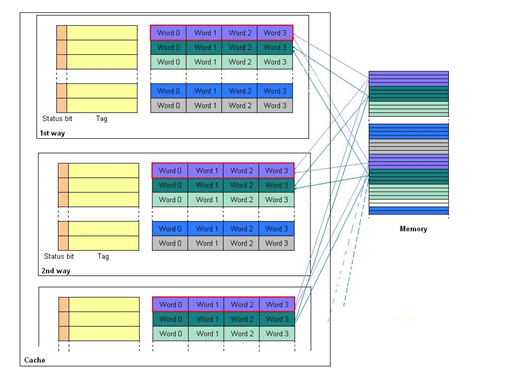
\includegraphics[scale=0.7]{fig4}}
		\caption{Схема памяти с множественно-ассоциативным отображением}
	\end{figure}
	\newpage
	\newpage
	\subsection{Замещение информации в кэш-памяти}
	\subsection{Запись в кэш-память}
	При возникновении промаха контроллер кэш-памяти должен выбрать подлежащую замещению строку. Для с прямого отображения аппаратные решения наиболее простые. На попадание проверяется только одна строка, и только эта строка может быть замещена. При полностью ассоциативной или множественно-ассоциативной организации кэш-памяти имеются несколько строк, из которых надо выбрать кандидата в случае промаха. Для решения этой задачи используют следующие специальные правила, называемые алгоритмами замещения.

1) FIFO (First In First Out – первый пришедший – первым выбывает);

2) LRU (Least Recently Used – дольше других неиспользуемый), а также возможные его разнеовидности - PLRU, SLRU и т.д.;

3) LFU (Least Frequently Used – реже других используемый);

4) Случайный (random).

Первый и последний методы являются самыми простыми в реализации, но они не учитывают, насколько часто используется та или иная строка КЭШ-памяти. При этом может быть удалена строка, к которой в самом ближайшем будущем будет обращение. Вероятность ошибки для указанных методов гораздо выше, чем у второго и третьего.

В алгоритме FIFO для замещения выбирается строка, первой попавшая в кэш. Каждая вновь размещаемая в кэше строка добавляется в конец этой очереди. Алгоритм не учитывает фактическое ее использование. Например, первые загруженные строки могут содержать данные, требующиеся на протяжении всей работы. Это приводит к немедленному возвращению к только что замещенной строке.

Алгоритм LRU предусматривает, что для удаления следует выбирать ту строку, которая не использовалась дольше других. При каждом обращении к строке ее временная метка обновляется. Это может быть сопряжено с существенными издержками. Однако алгоритм LRU наиболее часто используется на практике. Недостаток его заключается в том, что если программа проходит большой цикл, охватывающий множество строк, может случиться так, что строка, к которой дольше всего не было обращений, в действительности станет следующей используемой.

Одним из близких к LRU является алгоритм LFU, согласно которому удаляется наименее часто использовавшаяся строка. При этом необходимо подсчитывать количество обращений к каждой строке и контролировать его. Может оказаться, что наименее интенсивно используется та строка, которая только что записана в КЭШ-память и к которой успели обратиться только один раз (в то время как к другим строкам обращались больше). Она может быть удалена, что является недостатком алгоритма LFU.

Содержимое кэш-памяти меняется под управлением процессора. При этом основная память может оставаться неизменной. С другой стороны, внешние устройства могут изменять данные в ОП в режиме прямого доступа. При этом кэш-память не меняет своих данных. Еще сложнее ситуация в мультипроцессорных системах, когда несколько процессоров обращаются к общей памяти. Возникает проблема когерентности кэш-памяти.

Вычислительная система имеет когерентную память, если каждая операция чтения по адресу, выполненная каким-либо устройством, возвращает значение последней копии по этому адресу, независимо от того, какое из них производило запись последним. Проблема когерентности является наиболее важной для систем с обратным копированием. В них используются специальные протоколы, а к каждому тегу добавляются флаги модифицированности и достоверности информации. Эти флаги разрешают доступ к данным или запрещают его.
	\subsubsection{Сквозная (прямая) запись}\\
    При сквозной записи обновляется слово, хранящееся в основной памяти. Если в кэш-памяти существует копия данного слова, то она также обновляется. Если в кэш-памяти отсутствует копия данного слва, то из основной памяти пересылается блок, содержащий обновленное слово.\\
    Достоинство: если блок данных вытесняется, то нет необходимости возвращать его в ОЗУ, поскольку его копия там имеется.\\
    Недостаток: отсутствует прирост производительности при выполнении операций записи.
	\subsubsection{Отложенная (обратная) запись}\\
	В этом случае:\\
        - слово заносится только в кэш-память; \\
        - если соответствующего блока в кэш-памяти нет, то блок вначале пересылается из основной памяти, после чего запись все равно выполняется исключительно в кэш-память; \\
        - при замещении блока его необходимо предварительно переслать в соответствующее место основной памяти; \\
        - при каждом чтении из основной памяти осуществляются две пересылки между основной и кэш-памятью. 

Разновидность метода обратной записи – метод флаговой обратной записи. При изменении в каком-то блоке кэш-памяти устанавливается связанный с этим блоком бит изменения (флаг). Когда производится замещение блока, то он переписывается в основную память только тогда, когда его флаг установлен в 1. Разумеется, эффективность флаговой записи несколько выше. \cite{book:33863}
	\newpage
	\section{Реализация кэш-памяти}
	\subsection{Техническое задание}
	\textbf{Цель работы:} изучение основ структурного проектирования вычислительных систем, овладение современными САПР, получение навыков патентного поиска и исследовательской деятельности.\\
	
	1. Необходимо разработать систему памяти, включающую в себя кэш-память заданного размера. Система памяти должна принимать запросы на чтение/запись со стороны системной шины, выполнять поиск запрошенных данных в кэш-памяти. В случае кэш-промаха - перенаправлять запрос в контроллер оперативной памяти. Результаты запроса должны сохраняться в кэш, при необходимости вытеснив более старые данные в соответствии с заданным алгоритмом вытеснения. В случае кэш-попадания или после получения данных из ОП на запрос системной шины должен быть сформирован корректный ответ. Параметры системы памяти приведены в таблице 1.\\
	Системная шина, кэш память и интерфейс с ОП находятся в различных тактовых доменах.\\
	Интерфейс с \textbf{системной шиной} включает в себя следующие сигналы:
	
	\hspace{5mm}Входы: \textit{sys\_clk, sys\_rst\_n, sys\_addr[15:0], sys\_wr, sys\_rd, sys\_wdata[31:0], sys\_bval[31:0]}
	
	\hspace{5mm}Выходы: \textit{sys\_rdata[31:0], sys\_ack}\\
	Интерфейс с \textbf{контроллером оперативной памяти} включает в себя следующие сигналы:
	
	\hspace{5mm}Входы: \textit{ram\_clk, ram\_rst\_n, ram\_rdata[\textbf{31}:0], ram\_rack}
	
	\hspace{5mm}Выходы: \textit{ram\_addr[\textbf{11}:0], ram\_wdata[\textbf{31}:0], ram\_avalid, ram\_rnw}\\
	
	2. Провести патентный поиск по изобретениям и полезным моделям с глубиной поиска 25 лет (1994-2019) по заданным в таблице 1 алгоритмам и странам. Отчёт по поиску оформить в соответствии с ГОСТ Р 15.011-906, в т.ч. аналитическая часть. Таблица В.6.1, в приложении рефераты патентов.\\\\
	\begin{tabular}{ | p{200pt} | p{220pt} |}
	\hline
	Тип кэш-памяти & 8-ми канальная \\ \hline
	Объем кэш-памяти, байт & 2048 \\ \hline
    Разрядность шины данных ОП, байт & 4 \\ \hline
	Разрядность строки кэш-памяти, байт & 16 \\ \hline
	Алгоритм вытеснения & SLRU \\ \hline
	Алгоритм записи & прямая \\ \hline
	Алгоритмы для патентного поиска & записи \\ \hline
	Страны для патентного поиска & Россия, Франция, США \\ \hline
    \end{tabular}
    \begin{center}Таблица 1 --- Параметры задания (вариант 13)\end{center} \\\\
    Этапы выполнения работы:
    
    1. Подготовить обзор кэш-памяти;        
    
    2. Выполнить проектирование системы памяти;
    
    3. Провести патентный поиск;
    
    4. Подготовить пояснительную записку по выполненной работе.\\\\
    Базы данных для патентного поиска:\\\\
    \begin{tabular}{ | p{200pt} | p{220pt} |}
	\hline
	Роспатента & http://www.fips.ru \\ \hline
	ЕПВ Espacenet & http://ep.espacenet.com \\ \hline
    США USPATEULL & http://www.uspto.gov \\ \hline
	Google Patent Search & http://www.google.com/patent \\ \hline
	Всемирная организация интеллектуальной собственности (ВОИС) в системе PATENSCOPE & http://patentscope.wipo.int/search/en/search.jsf \\ \hline
    \end{tabular} 
    \newpage
	\subsection{Общее описание}
	
	В процессе проектирования системы памяти были выполнены следующие задачи:
	
	1. Разработаны алгоритмы функционирования памяти тэгов, устройства управления, схемы замещения, алгоритмы чтения и записи в память;
	
	2. Разработана функциональная схема системы памяти и её компонентов согласно алгоритмам;
	
	3. Реализована система памяти на языке Verilog. Система памяти состоит из следующих компонентов:
	
	- Модуль взаимодействия с CPU;\\
	- Память тэгов;\\
	- Память данных;\\
	- Контроллер системы памяти;\\
	- Модуль взаимодействия с RAM;\\
	
	4. Разработаны тесты компонентов, а также интеграционные тесты системы памяти на языке SystemVerilog.\\
	\subsubsection{Особенности реализации}
	Исходя из технического задания, ниже выведены детальные параметры подсистемы памяти.\\
	1. $\cfrac{2048\ bytes}{16\ bytes} = 128$ строк содержится в кэш-памяти.\\
	2. $\cfrac{128\ rows}{8\ channels} = 16$ банков памяти содержит кэш-память. В каждом банке хранится 8 строк.\\
	3. $size(offset) = \log_216 = 4$ бита требуется для адресации одного байта в строке.\\
	4. $size(index) = \log_216 = 4$ бита требуется для адресации банка памяти.\\
	5. $size(tag) = 16-4-4 = 8$ бит требуется для тэга.
	
	На рисунках 5 и 6 приведены основные алгоритмы работы кэш-памяти.
	\newpage
	\subsection{Алгоритмы работы кэш-памяти}\\
	\begin{figure}[h!]
		\center{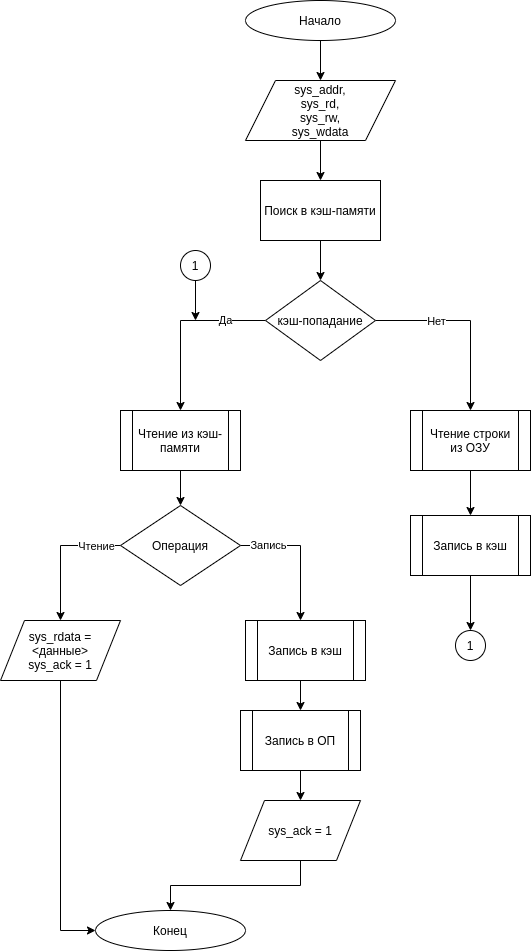
\includegraphics[scale=0.5]{cache_algo.png}}
		\caption{Блок-схема общего алгоритма работы кэш-памяти}
	\end{figure}\\
	\begin{figure}[h!]
		\center{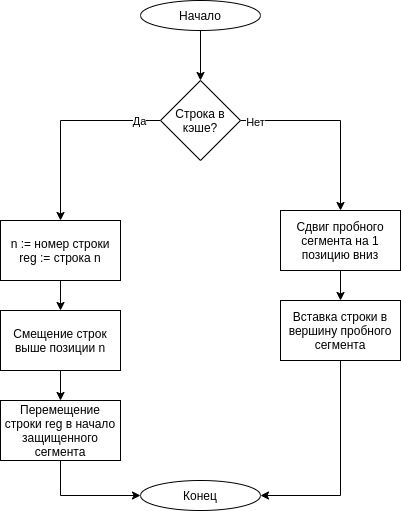
\includegraphics[scale=0.5]{slru_algo.png}}
		\caption{Блок-схема работы алгоритма вытеснения SLRU}
	\end{figure}
	\newpage
	\subsection{Функциональная схема}
	Функциональная схема кэш-памяти приведена на рисунке 7.
	\begin{figure}[h!]
		\center{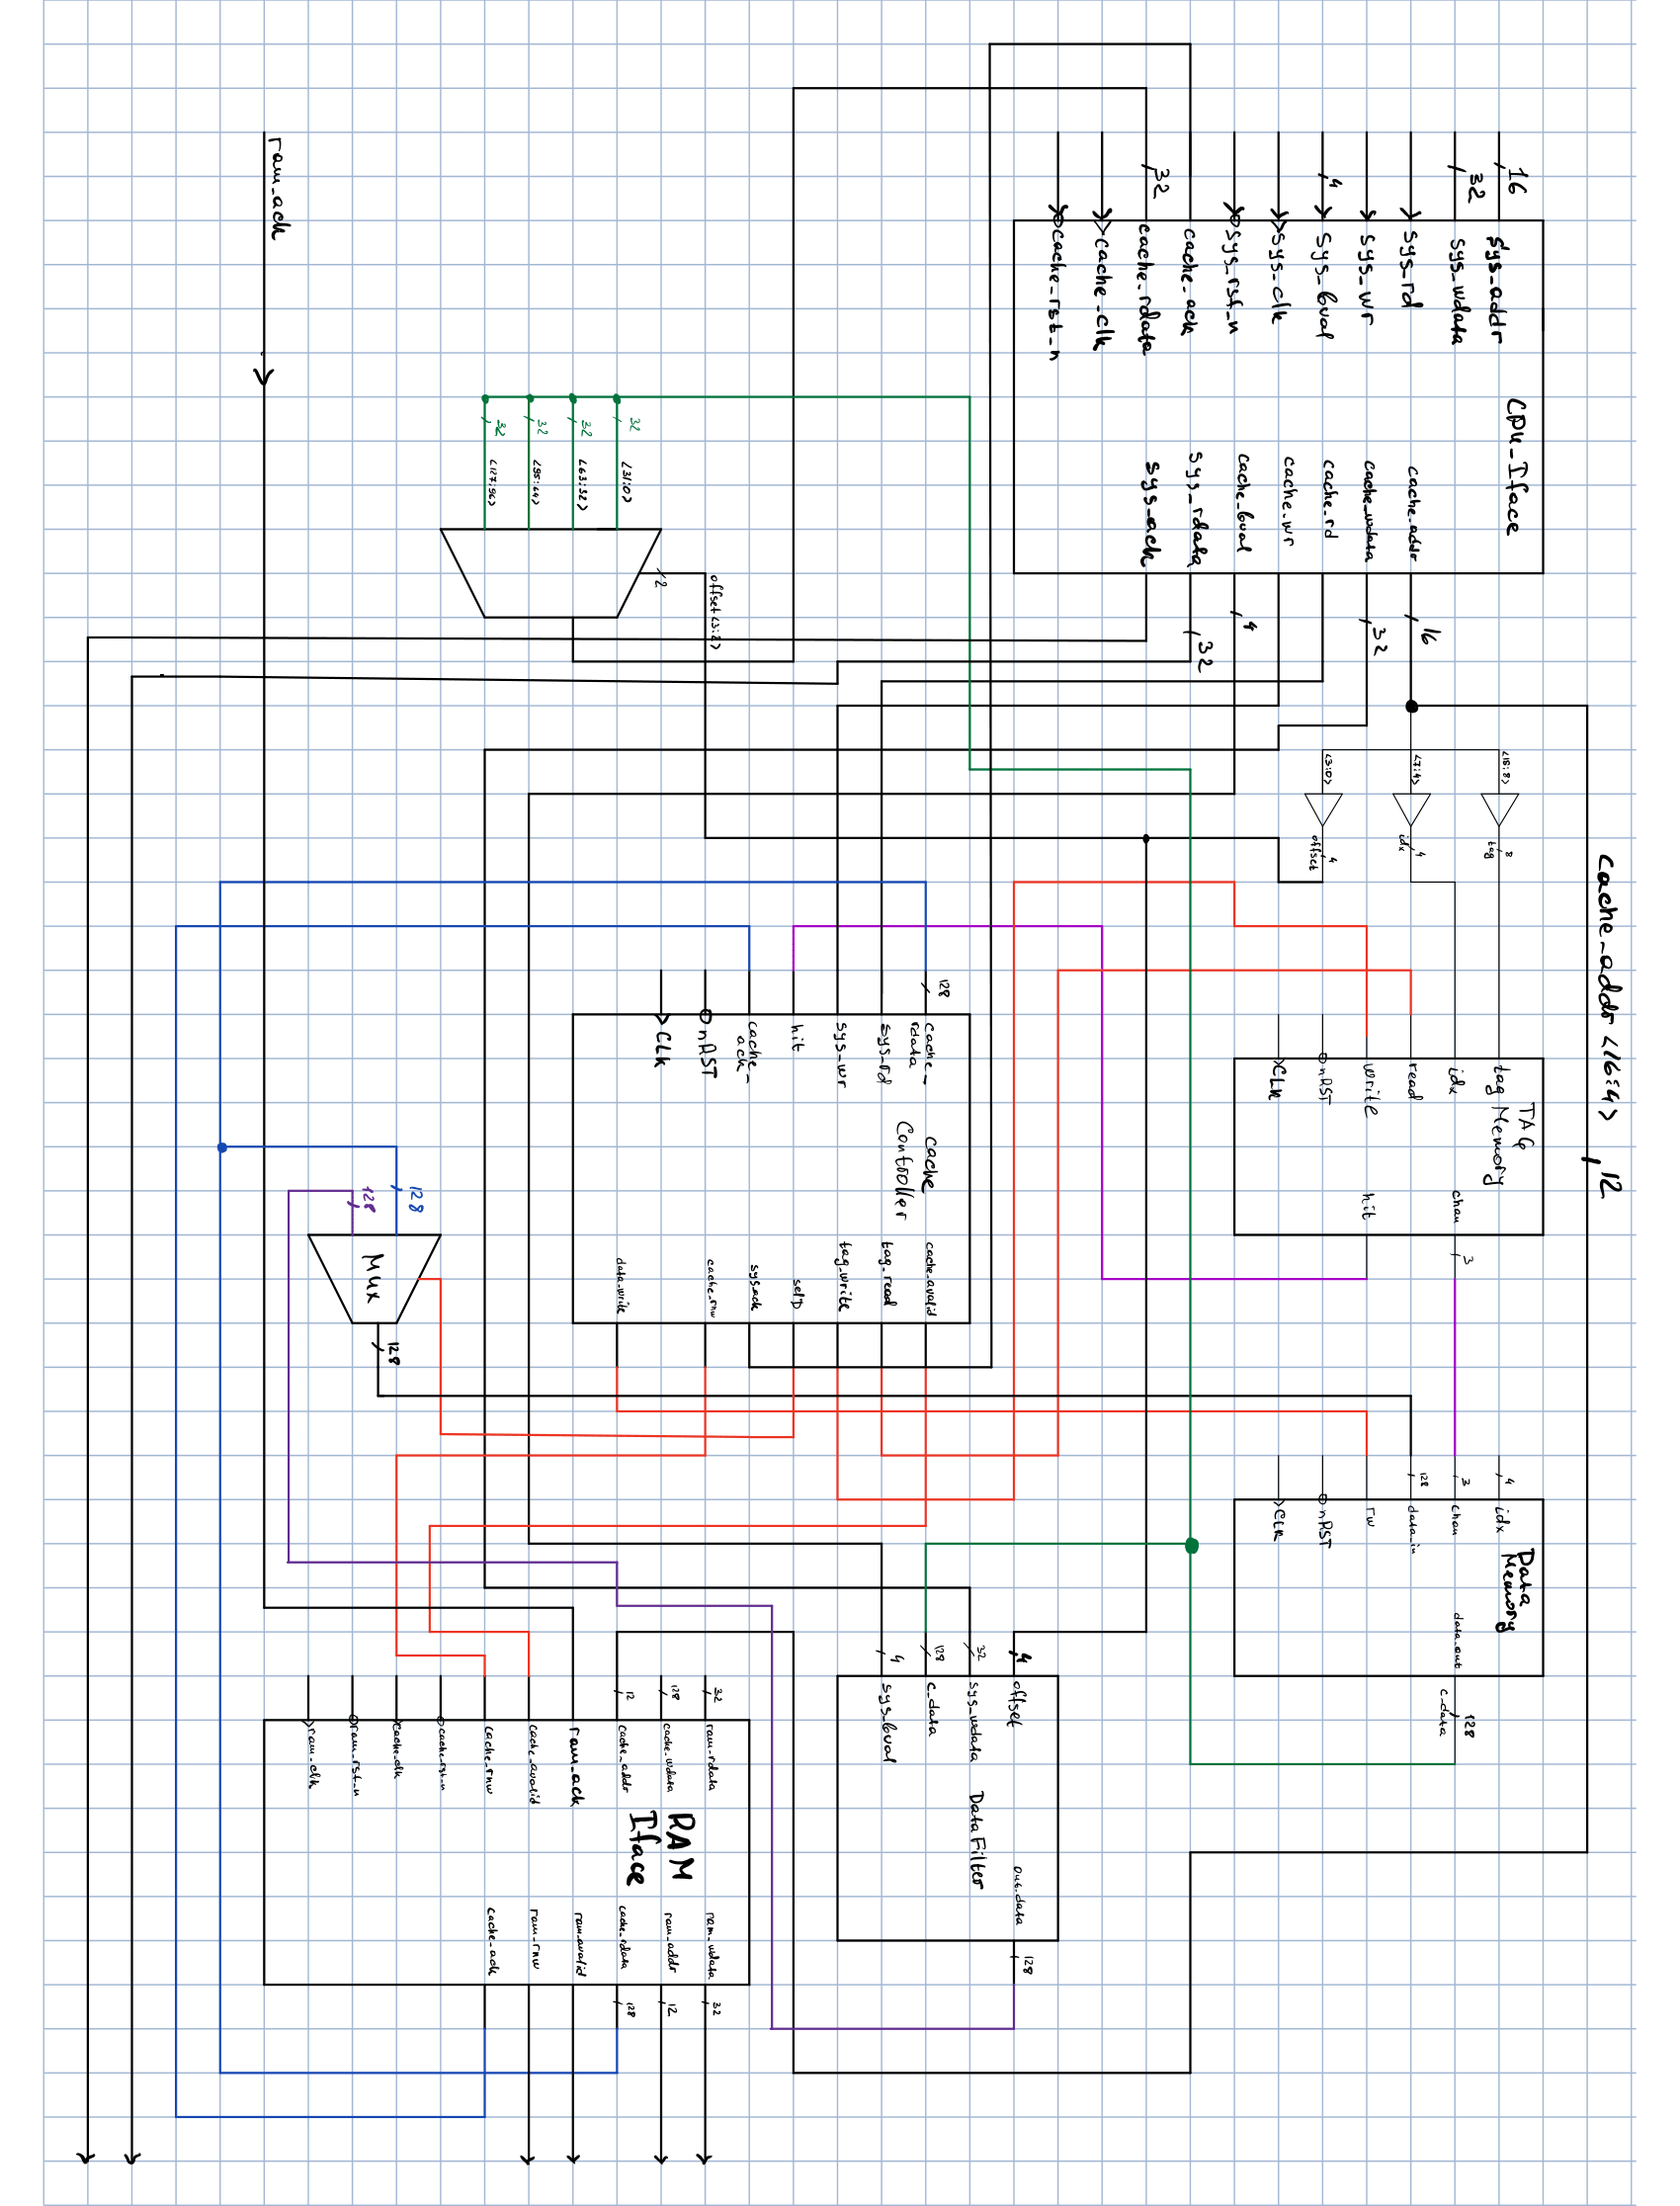
\includegraphics[scale=0.3]{scheme.png}}
		\caption{Функциональная схема кэш-памяти}
	\end{figure}
	\newpage
	\subsection{Описание модулей и особенности реализации}
	\subsubsection{Модуль взаимодействия с CPU}
	\begin{center}
	\begin{circuitikz}
    \ctikzset{multipoles/thickness=3}
    \ctikzset{multipoles/dipchip/width=4}
    \draw (0,0) node[dipchip,
    num pins=26, hide numbers, no topmark,
    external pins width=0](C){CPU\_IFACE};
    \node [right, font=\tiny] at (C.bpin 1) {sys\_addr<15:0>};
    \node [right, font=\tiny] at (C.bpin 2) {sys\_wdata<31:0>};
    \node [right, font=\tiny] at (C.bpin 3) {sys\_bval<3:0>};
    \node [right, font=\tiny] at (C.bpin 4) {cache\_rdata<31:0>};
    \node [right, font=\tiny] at (C.bpin 6) {sys\_rd};
    \node [right, font=\tiny] at (C.bpin 7) {sys\_wr};
    \node [right, font=\tiny] at (C.bpin 8) {sys\_clk};
    \node [right, font=\tiny] at (C.bpin 9) {sys\_rst\_n};
    \node [right, font=\tiny] at (C.bpin 10) {cache\_clk};
    \node [right, font=\tiny] at (C.bpin 11) {cache\_rst\_n};
    \node [right, font=\tiny] at (C.bpin 12) {cache\_ack};
    
    \node [left, font=\tiny] at (C.bpin 15) {sys\_rdata<31:0>};
    \node [left, font=\tiny] at (C.bpin 16) {cache\_addr<15:0>};
    \node [left, font=\tiny] at (C.bpin 17) {cache\_wdata<31:0>};
    \node [left, font=\tiny] at (C.bpin 18) {cache\_bval<3:0>};
    \node [left, font=\tiny] at (C.bpin 19) {sys\_ack};
    \node [left, font=\tiny] at (C.bpin 20) {cache\_rd};
    \node [left, font=\tiny] at (C.bpin 21) {cache\_wr};
    \draw (C.bpin 1) -- ++(-0.5,0) coordinate(extpin);
    \draw (C.bpin 2) -- ++(-0.5,0) coordinate(extpin);
    \draw (C.bpin 3) -- ++(-0.5,0) coordinate(extpin);
    \draw (C.bpin 4) -- ++(-0.5,0) coordinate(extpin);
    \draw (C.bpin 6) -- ++(-0.5,0) coordinate(extpin);
    \draw (C.bpin 7) -- ++(-0.5,0) coordinate(extpin);
    \draw (C.bpin 8) -- ++(-0.5,0) coordinate(extpin);
    \draw (C.bpin 9) -- ++(-0.5,0) coordinate(extpin);
    \draw (C.bpin 10) -- ++(-0.5,0) coordinate(extpin);
    \draw (C.bpin 11) -- ++(-0.5,0) coordinate(extpin);
    \draw (C.bpin 12) -- ++(-0.5,0) coordinate(extpin);
    
    \draw (C.bpin 15) -- ++(0.5,0) coordinate(extpin);
    \draw (C.bpin 16) -- ++(0.5,0) coordinate(extpin);
    \draw (C.bpin 17) -- ++(0.5,0) coordinate(extpin);
    \draw (C.bpin 18) -- ++(0.5,0) coordinate(extpin);
    \draw (C.bpin 19) -- ++(0.5,0) coordinate(extpin);
    \draw (C.bpin 20) -- ++(0.5,0) coordinate(extpin);
    \draw (C.bpin 21) -- ++(0.5,0) coordinate(extpin);
    % inverse to pin
    %\node [ocirc, anchor=0](notin2) at (C.bpin 2) {};
    %\draw (notin2.180) -- (C.bpin 2 -| extpin);
    
    %\node [ocirc, anchor=0](notin2) at (C.bpin 7) {};
    %\draw (notin2.180) -- (C.bpin 7 -| extpizn);
    
    \draw (C.bpin 10) ++(0,0.1) -- ++(0.1,-0.1)
    node[right, font=\tiny] -- ++(-0.1,-0.1);
    
    \draw (C.bpin 8) ++(0,0.1) -- ++(0.1,-0.1)
    node[right, font=\tiny] -- ++(-0.1,-0.1);
    \end{circuitikz}
    \end{center}
    \begin{figure}[h!]
		\caption{УГО модуля взаимодействия с CPU}
	\end{figure}\\
	Модуль взаимодействия с CPU отвечат за перевод данных, приходящих от CPU по синхросигналу sys\_clk, в частотный домен, который управляется синхросигналом кэш-памяти (cache\_clk). И наоборот.\\
	\textbf{Входы:}\\
	- sys\_addr - адрес, приходящий от CPU;\\
	- sys\_wdata - данные для записи, приходящие от CPU;\\
	- sys\_bval - сигналы, определяющие, какие байты в слове будут перезаписаны;\\
	- cache\_rdata - прочитанные данные, приходящие из кэш-памяти;\\
	- sys\_rd - сигнал чтения, приходящий из CPU;\\
	- sys\_wr - сигнал записи, приходящий из CPU;\\
	- sys\_clk - синхросигал CPU;\\
	- sys\_rst\_n - асинхронный сброс, приходящий из CPU;\\
	- cache\_clk - собственный синхросигнал кэш-памяти;\\
	- cache\_rst\_n - собственный сигнал асинхронного сброса кэш-памяти;\\
	- cache\_ack - сигнал подтверждения, приходящий из кэш-памяти.\\
	\textbf{Выходы:}\\
	- cache\_wr - сигнал sys\_rw, переведённый в частотный домен кэш-памяти;\\
	- cache\_rd - сигнал sys\_rd, переведённый в частотный домен кэш-памяти;\\
	- sys\_ack - сигнал cache\_ack, переведённый в частотный домен CPU;\\
	- cache\_bval - сигнал sys\_bval, переведённый в частотный домен кэш-памяти;\\
	- cache\_wdata - сигнал sys\_wdata, переведённый в частотный домен кэш-памяти;\\
	- cache\_addr - сигнал sys\_addr, переведённый в частотный домен кэш-памяти;\\
	- sys\_rdata - данные регистра cache\_rdata, переведённые в частотный домен CPU;\\
	
	\subsubsection{Память тэгов}
	Модуль памяти тегов отвечает за хранение тегов, а также обеспечивает вытеснение данных в случае, если кэш-память заполнена. УГО модуля приведено на рисунке 5.\\
	\begin{figure}[h!]
    	\begin{center}
        	\begin{circuitikz}
                \ctikzset{multipoles/thickness=3}
                \ctikzset{multipoles/dipchip/width=4}
                \draw (0,0) node[dipchip,
                num pins=12, hide numbers, no topmark,
                external pins width=0](C){TAG\_MEM};
                \node [right, font=\tiny] at (C.bpin 1)     {tag<7:0>};
                \node [right, font=\tiny] at (C.bpin 2)     {idx<3:0>};
                \node [right, font=\tiny] at (C.bpin 3)     {CLK};
                \node [right, font=\tiny] at (C.bpin 4)     {nRST};
                \node [right, font=\tiny] at (C.bpin 5)     {rd};
                \node [right, font=\tiny] at (C.bpin 6)     {wr};
                \node [right, font=\tiny] at (C.bpin 9)     {chan<2:0>};
                \node [right, font=\tiny] at (C.bpin 11)    {hit};
                
                \draw (C.bpin 1) -- ++(-0.5,0) coordinate(extpin);
                \draw (C.bpin 2) -- ++(-0.5,0) coordinate(extpin);
                \draw (C.bpin 3) -- ++(-0.5,0) coordinate(extpin);
                \draw (C.bpin 4) -- ++(-0.5,0) coordinate(extpin);
                \draw (C.bpin 5) -- ++(-0.5,0) coordinate(extpin);
                \draw (C.bpin 6) -- ++(-0.5,0) coordinate(extpin);
                \draw (C.bpin 9) -- ++(-0.5,0) coordinate(extpin);
                \draw (C.bpin 10) -- ++(-0.5,0) coordinate(extpin);
                \draw (C.bpin 11) -- ++(-0.5,0) coordinate(extpin);
                
                \draw (C.bpin 3) ++(0,0.1) -- ++(0.1,-0.1)
                node[right, font=\tiny] -- ++(-0.1,-0.1);
            \end{circuitikz}
    	\end{center}
    	\caption{УГО памяти тэгов}
	\end{figure}\\
	\textbf{Входы:}\\
	- CLK - вход синхронизации;\\
	- nRST - вход асинхронного сброса;\\
	- tag - тэг;\\
	- idx - индекс;\\
	- read - режим работы: чтение;\\
	- write - режим работы: запись.\\\\
	\textbf{Выходы:}\\
	- hit - сигнал, который устанавливается в 1 в случае кэш-попадания;\\
	- chan - номер канала, в котором обнаружено кэш-попадание.\\
	
	\subsubsection{Память данных}
	Модуль памяти данных отвечает за хранение данных в секции, определяемой индексов и канале, который определяется памятью тегов. УГО представлено на рисунке 10.\\
    \begin{figure}[h!]
    	\begin{center}
        	\begin{circuitikz}
                \ctikzset{multipoles/thickness=3}
                \ctikzset{multipoles/dipchip/width=4}
                \draw (0,0) node[dipchip,
                num pins=12, hide numbers, no topmark,
                external pins width=0](C){DATA\_MEM};
                \node [right, font=\tiny] at (C.bpin 1)     {CLK};
                \node [right, font=\tiny] at (C.bpin 2)     {idx<3:0>};
                \node [right, font=\tiny] at (C.bpin 3)     {nRST};
                \node [right, font=\tiny] at (C.bpin 4)     {chan<2:0>};
                \node [right, font=\tiny] at (C.bpin 5)     {data\_in<127:0>};
                \node [right, font=\tiny] at (C.bpin 6)     {rw};
                \node [right, font=\tiny] at (C.bpin 10)    {data\_out<127:0>};
                
                \draw (C.bpin 1) -- ++(-0.5,0) coordinate(extpin);
                \draw (C.bpin 2) -- ++(-0.5,0) coordinate(extpin);
                \draw (C.bpin 3) -- ++(-0.5,0) coordinate(extpin);
                \draw (C.bpin 4) -- ++(-0.5,0) coordinate(extpin);
                \draw (C.bpin 5) -- ++(-0.5,0) coordinate(extpin);
                \draw (C.bpin 6) -- ++(-0.5,0) coordinate(extpin);
                \draw (C.bpin 10) -- ++(-0.5,0) coordinate(extpin);
                
                \draw (C.bpin 1) ++(0,0.1) -- ++(0.1,-0.1)
                node[right, font=\tiny] -- ++(-0.1,-0.1);
            \end{circuitikz}
    	\end{center}
    	\caption{УГО памяти тэгов}
	\end{figure}\\

	\textbf{Входы:}\\
	- CLK - вход синхронизации;\\
	- nRST - вход асинхронного сброса;\\
	- idx - индекс;\\
	- chan - канал, в который выполняется запись;\\
	- rw - режим чтения (0) или записи (1);\\
	- data\_in - входные данные для записи;\\
	\textbf{Выходы:}\\
	- data\_out - выходные, прочитанные данные;\\
	\subsubsection{Контроллер кэш-памяти}
			\begin{figure}[h!]
    	\begin{center}
        	\begin{circuitikz}
                \ctikzset{multipoles/thickness=3}
                \ctikzset{multipoles/dipchip/width=4}
                \draw (0,0) node[dipchip,
                num pins=16, hide numbers, no topmark,
                external pins width=0](C){Controller};
                \node [right, font=\tiny] at (C.bpin 1)     {cache\_rdata<127:0>};
                \node [right, font=\tiny] at (C.bpin 2)     {CLK};
                \node [right, font=\tiny] at (C.bpin 3)     {nRST};
                \node [right, font=\tiny] at (C.bpin 4)     {sys\_rd};
                \node [right, font=\tiny] at (C.bpin 5)     {sys\_wr};
                \node [right, font=\tiny] at (C.bpin 6)     {hit};
                \node [right, font=\tiny] at (C.bpin 7)     {cache\_ack};
                \node [right, font=\tiny] at (C.bpin 8)     {cache\_avalid};
                \node [right, font=\tiny] at (C.bpin 9)     {tag\_read};
                \node [right, font=\tiny] at (C.bpin 10)    {tag\_write};
                \node [right, font=\tiny] at (C.bpin 11)    {selD};
                \node [right, font=\tiny] at (C.bpin 12)     {sys\_ack};
                \node [right, font=\tiny] at (C.bpin 13)     {cache\_rnw};
                \node [right, font=\tiny] at (C.bpin 14)     {tag\_write\_en};
                \node [right, font=\tiny] at (C.bpin 15)     {data\_write};
                
                \draw (C.bpin 1) -- ++(-0.5,0) coordinate(extpin);
                \draw (C.bpin 2) -- ++(-0.5,0) coordinate(extpin);
                \draw (C.bpin 3) -- ++(-0.5,0) coordinate(extpin);
                \draw (C.bpin 4) -- ++(-0.5,0) coordinate(extpin);
                \draw (C.bpin 5) -- ++(-0.5,0) coordinate(extpin);
                \draw (C.bpin 6) -- ++(-0.5,0) coordinate(extpin);
                \draw (C.bpin 7) -- ++(-0.5,0) coordinate(extpin);
                \draw (C.bpin 8) -- ++(-0.5,0) coordinate(extpin);
                \draw (C.bpin 9) -- ++(-0.5,0) coordinate(extpin);
                \draw (C.bpin 10) -- ++(-0.5,0) coordinate(extpin);
                \draw (C.bpin 11) -- ++(-0.5,0) coordinate(extpin);
                \draw (C.bpin 12) -- ++(-0.5,0) coordinate(extpin);
                \draw (C.bpin 13) -- ++(-0.5,0) coordinate(extpin);
                \draw (C.bpin 14) -- ++(-0.5,0) coordinate(extpin);
                \draw (C.bpin 15) -- ++(-0.5,0) coordinate(extpin);
                
                \draw (C.bpin 2) ++(0,0.1) -- ++(0.1,-0.1)
                node[right, font=\tiny] -- ++(-0.1,-0.1);
            \end{circuitikz}
    	\end{center}
    	\caption{УГО кэш-контроллера}
	\end{figure}\\

    \begin{tikzpicture}[->, >=stealth', shorten >=1pt, auto, node    distance=4cm,thick, main node/.style={circle, draw, font=\sffamily\Large}]
    \node[initial right, state] (S1) {$IDLE$};
    \node[state] (S2) [below=of S1] {$RRAM$};
    \node[state] (S7) [below=of S2] {$WAIT$};
    \node[state] (S3) [left=of S1] {$SELECT$};
    \node[state] (S4) [below left=of S3] {$ACK$};
    \node[state] (S5) [right=2cm of S4] {$WRITE_{CR}$};
    \node[state] (S6) [left= 2cm of S2] {$WRITE_C$};
    
    \path[every node/.style={font=\sffamily\small}, label distance=9pt]
        (S1) edge [above] node[above=4pt] {$hit\And(sys\_rd\oplus sys\_wr)$} (S3)
        (S1) edge  node[sloped] {$ hit = 0$} (S2)
        (S2) edge  node[sloped] {} (S7)
        (S7) edge  node[sloped] {$ram\_rack = 1$} (S6)
        (S6) edge  node {$ $} (S3)
        (S3) edge  node[above, sloped] {$Read$} (S4)
        (S3) edge  node[above, sloped] {$Write$} (S5)
        (S5) edge  node {$ $} (S4)
        (S4) edge  node {$ $} (S1); 
    \end{tikzpicture}\\
    \begin{figure}[h!]
		\caption{Граф состояний контроллера кэш-памяти}
	\end{figure}\\
    Описание состояний:\\
    - \textbf{IDLE} - начальное состояние. В этом состоянии кэш-память ожидает прихода операции.;\\
    - \textbf{SELECT} - выбор действия (чтение, запись). Переход осуществляется из состояния IDLE при условии кэш-попадания и выбора одного из режимов (чтение или запись), а также из ветви кэш-промаха после записи в кэш-память отсутствующих данных;\\
    - \textbf{RRAM} - чтение данных из RAM. Переход осуществляется из состояния IDLE при условии кэш-промаха и выбора одного из режимов (чтение или запись);\\
    - \textbf{WAIT} - ожидание данных из RAM. Переход осуществляется из состояния RRAM сразу. В этом состоянии кэш-память ожидает сигнала ram\_ack от ОЗУ.\\
    - \textbf{WRITE\_C} - запись отсутствующих данных в кэш-память. Переход осуществляется из состояния WAIT при возникновении сигнала подтверждения от ОЗУ о том, что данные прочитаны. В этом состоянии память записывает тэг в память тэгов, а также данные в память данных.\\
    - \textbf{WRITE\_CR} - запись данных в кэш-память и ОЗУ. Переход в это состояние осуществляется из состояния SELECT при операции записи. В этом состоянии кэш-память записывает модифицированные данные в память данных, а также формирует транзакцию записи в RAM.\\
    - \textbf{ACK} - Подтверждение конца транзакции. Переход в это состояние осуществляется из состояния SELECT при выборе операции чтения, а также из состояния WRITE\_CR, после того, как данные записаны в кэш и ОЗУ.
    

	\subsubsection{Модуль взаимодействия с ОЗУ}
	\begin{center}
    \begin{circuitikz}
    \ctikzset{multipoles/thickness=3}
    \ctikzset{multipoles/dipchip/width=4}
    \draw (0,0) node[dipchip,
    num pins=22, hide numbers, no topmark,
    external pins width=0](C){RAM\_IFACE};
    \node [right, font=\tiny] at (C.bpin 1) {ram\_clk};
    \node [right, font=\tiny] at (C.bpin 2) {ram\_rst\_n};
    \node [right, font=\tiny] at (C.bpin 3) {ram\_ack};
    \node [right, font=\tiny] at (C.bpin 4) {ram\_rdata<31:0>};
    \node [right, font=\tiny] at (C.bpin 6) {cache\_clk};
    \node [right, font=\tiny] at (C.bpin 7) {cache\_rst\_n};
    \node [right, font=\tiny] at (C.bpin 8) {cache\_rnw};
    \node [right, font=\tiny] at (C.bpin 9) {cache\_avalid};
    \node [right, font=\tiny] at (C.bpin 10) {cache\_addr<11:0>};
    \node [right, font=\tiny] at (C.bpin 11) {cache\_wdata<127:0>};
    
    \node [left, font=\tiny] at (C.bpin 15) {cache\_rdata<127:0>};
    \node [left, font=\tiny] at (C.bpin 16) {cache\_ack};
    \node [left, font=\tiny] at (C.bpin 17) {ram\_avalid};
    \node [left, font=\tiny] at (C.bpin 18) {ram\_rnw};
    \node [left, font=\tiny] at (C.bpin 19) {ram\_wdata<31:0>};
    \node [left, font=\tiny] at (C.bpin 20) {ram\_addr<11:0>};
    \draw (C.bpin 1) -- ++(-0.5,0) coordinate(extpin);
    \draw (C.bpin 2) -- ++(-0.5,0) coordinate(extpin);
    \draw (C.bpin 3) -- ++(-0.5,0) coordinate(extpin);
    \draw (C.bpin 4) -- ++(-0.5,0) coordinate(extpin);
    \draw (C.bpin 6) -- ++(-0.5,0) coordinate(extpin);
    \draw (C.bpin 7) -- ++(-0.5,0) coordinate(extpin);
    \draw (C.bpin 8) -- ++(-0.5,0) coordinate(extpin);
    \draw (C.bpin 9) -- ++(-0.5,0) coordinate(extpin);
    \draw (C.bpin 10) -- ++(-0.5,0) coordinate(extpin);
    \draw (C.bpin 11) -- ++(-0.5,0) coordinate(extpin);
    
    \draw (C.bpin 15) -- ++(0.5,0) coordinate(extpin);
    \draw (C.bpin 16) -- ++(0.5,0) coordinate(extpin);
    \draw (C.bpin 17) -- ++(0.5,0) coordinate(extpin);
    \draw (C.bpin 18) -- ++(0.5,0) coordinate(extpin);
    \draw (C.bpin 19) -- ++(0.5,0) coordinate(extpin);
    \draw (C.bpin 20) -- ++(0.5,0) coordinate(extpin);
    % inverse to pin
    %\node [ocirc, anchor=0](notin2) at (C.bpin 2) {};
    %\draw (notin2.180) -- (C.bpin 2 -| extpin);
    
    %\node [ocirc, anchor=0](notin2) at (C.bpin 7) {};
    %\draw (notin2.180) -- (C.bpin 7 -| extpizn);
    
    \draw (C.bpin 1) ++(0,0.1) -- ++(0.1,-0.1)
    node[right, font=\tiny] -- ++(-0.1,-0.1);
    
    \draw (C.bpin 6) ++(0,0.1) -- ++(0.1,-0.1)
    node[right, font=\tiny] -- ++(-0.1,-0.1);
    \end{circuitikz}
    \end{center}
    \begin{figure}[h!]
		\caption{УГО модуля взаимодействия с ОЗУ}
	\end{figure}
    Модуль взаимодействия с ОЗУ обеспечивает следующую функциональность:\\
    1. Обработку RAM-транзакций
    
    1.1 Формирование транзакций в корректном формате;
    
    1.2 Принятие транзакций от ОЗУ и обработку в кэш-памяти;\\
    2. Переход между частотными доменами.\\\\
    Модуль взаимодействия c ОЗУ управляется двумя синхросигналами:
    
    1. Синхросигнал кэш-памяти;
    
    2. Синхросигнал ОЗУ;\\
    
    \textbf{Общий принцип работы}. Согласно техническому заданию, размер строки кэш-памяти равен 16 байтам, а разрядность шины данных ОЗУ равна 4 байта. Возникают задачи сериализации и десериализации строки. Эти задачи решаются с помощью двух составляющих:
    
    1. Асинхронный модуль FIFO для чтения;
    
    2. Асинхронный модуль FIFO для записи;
    
    3. Регистр сдвига;
    
    4. Местное устройство управления, координирующее работу FIFO и регистра.
    
    Асинхронный модуль FIFO для чтения из ОЗУ управляется синхросигналом кэш-памяти (cache\_clk) для считывания данных в кэш и синхросигналом ОЗУ. Функциональная схема модуля взаимодействия приведена на рисунке 14.
    \newpage
	\begin{figure}[h!]
		\center{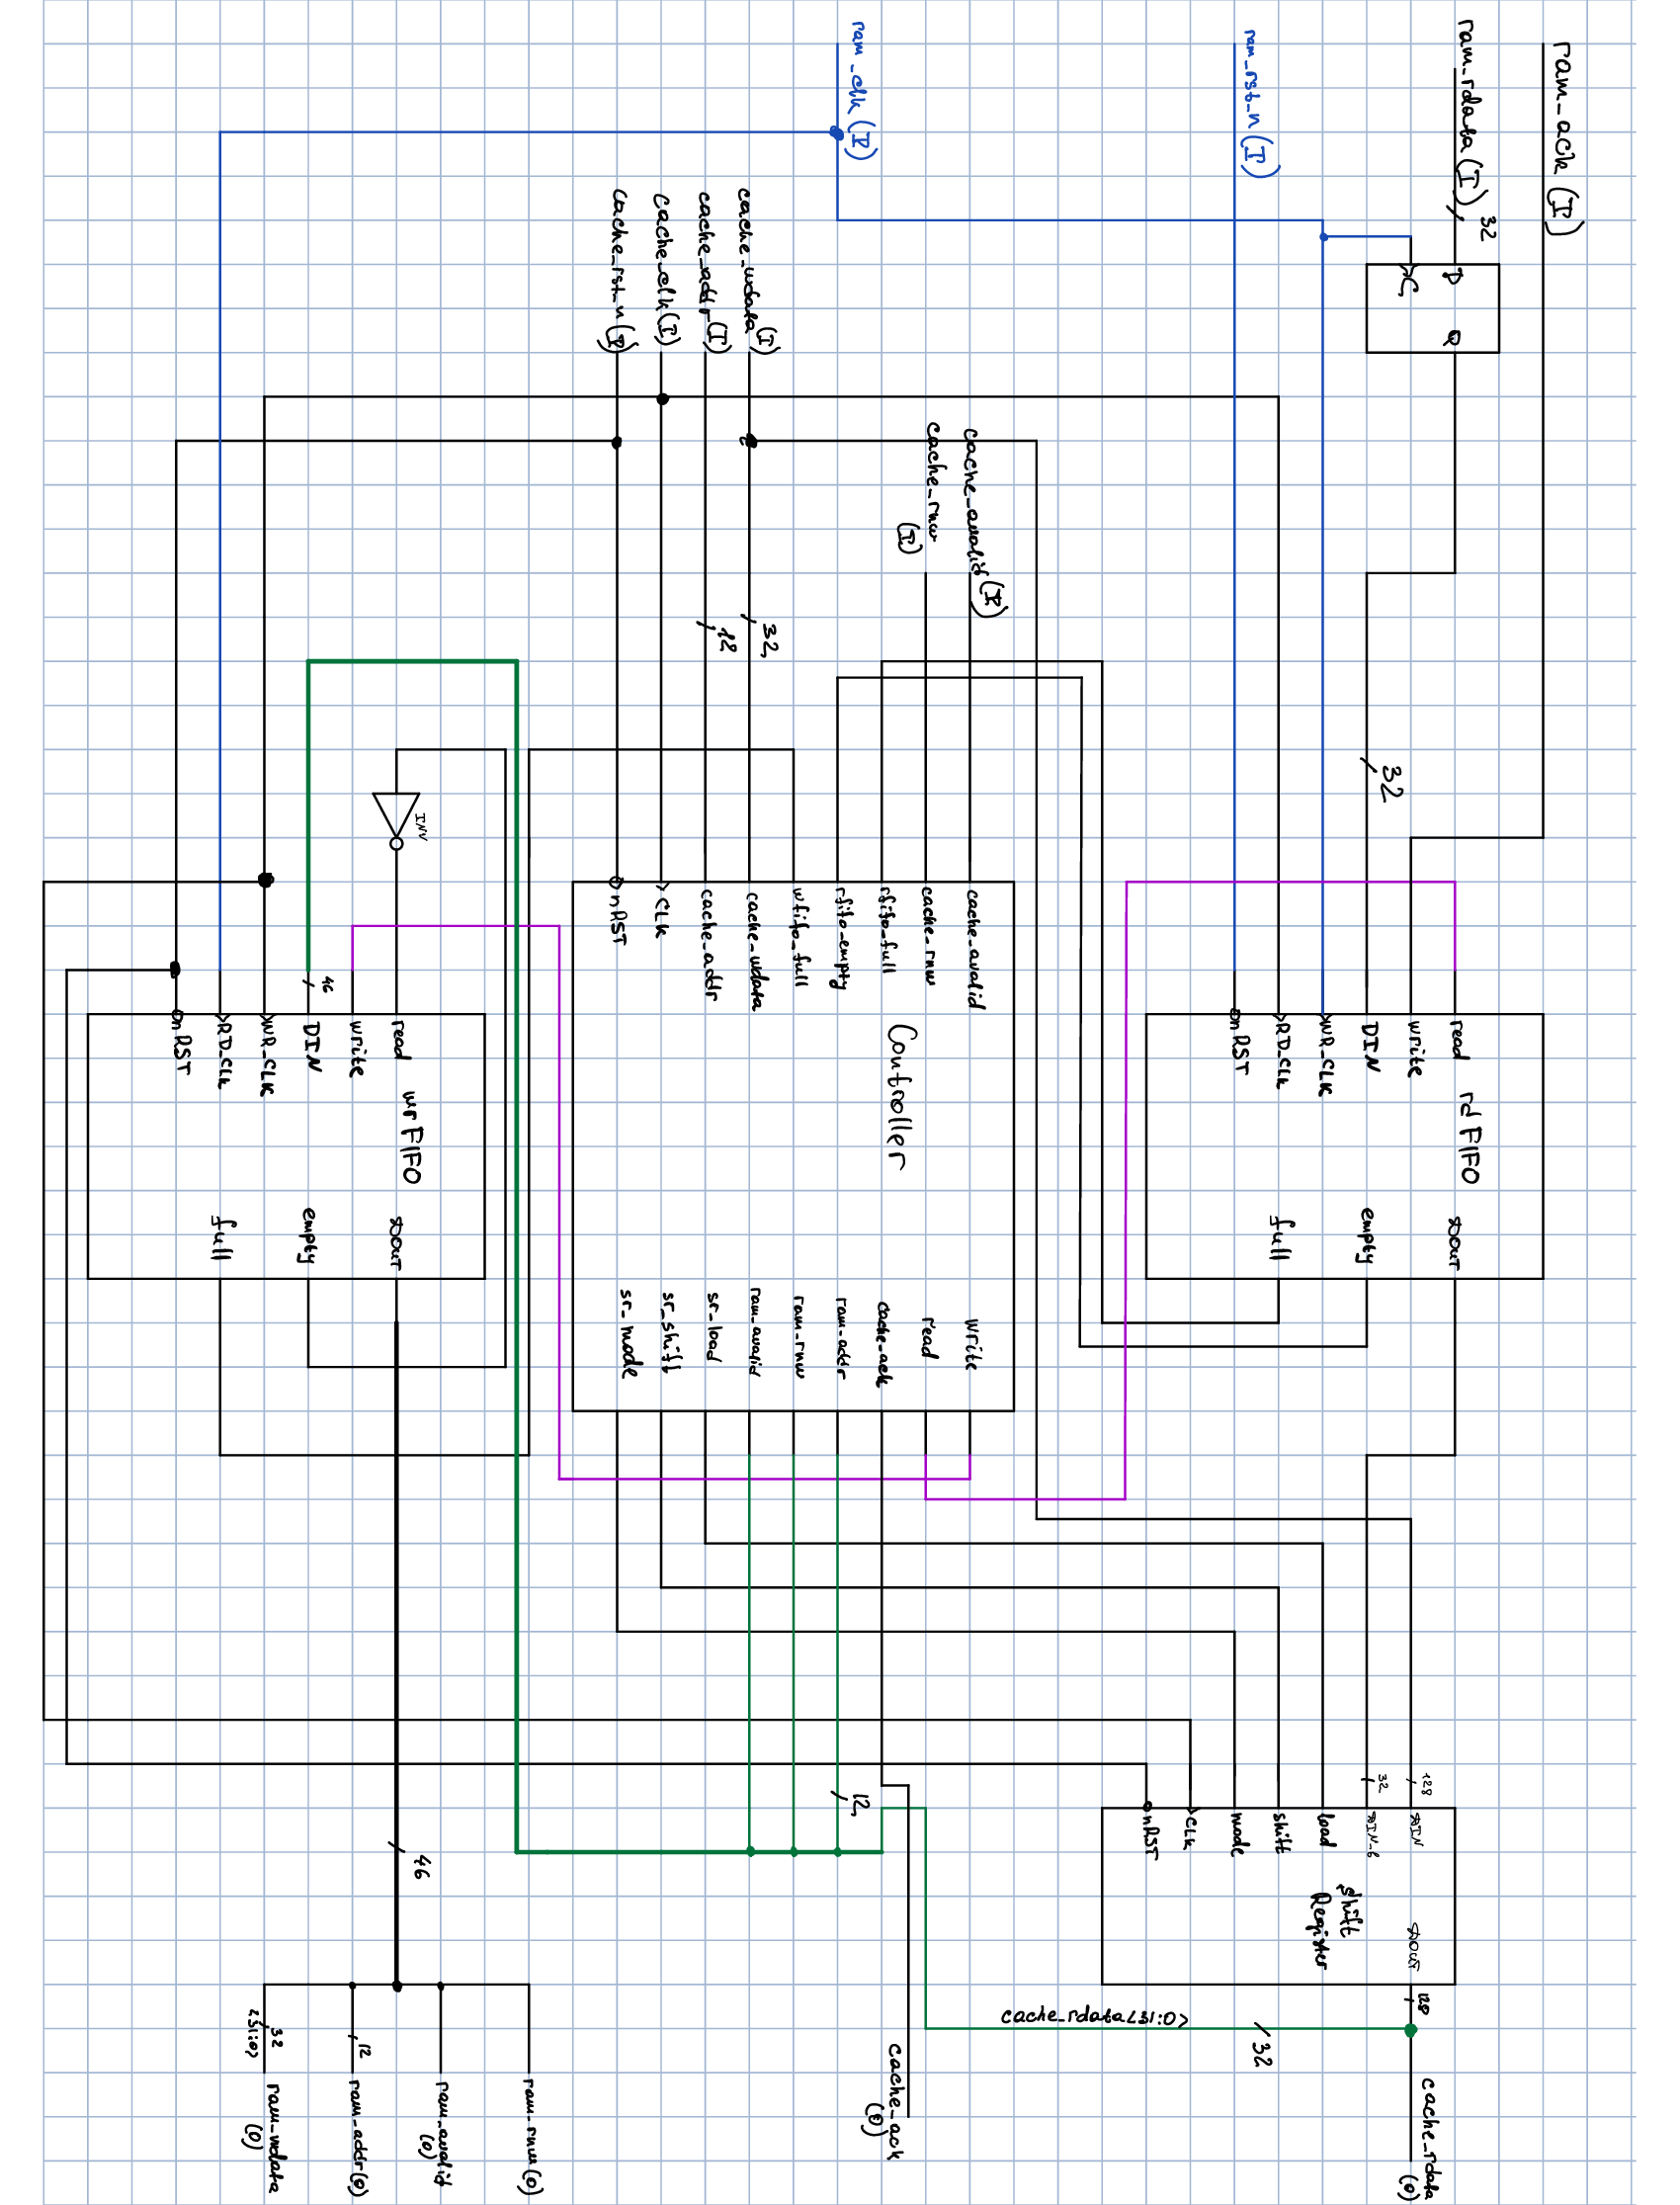
\includegraphics[scale=0.3]{ram_if_scheme.png}
		\caption{Функциональная схема модуля взаимодействия с ОЗУ}
	\end{figure}
	\newpage
	\setcounter{secnumdepth}{-1}
	\section{Заключение}
	Исходя из технического задания, была разработана система памяти, отвечающая всем заданным характеристикам. 
	
	Для того, чтобы разработать систему памяти, необходимо было понять, а какие типы кэш-памяти и какие архитектуры существуют. Для этого был проведён краткий обзор. Была составлена структура кэш-памяти, зависимость её характеристик от ёмкости и размера строки, были проанализированы существующие способы отображения, вытесенения и тип записи.
	
	На основе полученных данных был составлен алгоритм работы кэш-памяти, а также разработана функциональная схема устройства. Реализация системы памяти выполнена на языке описания аппаратуры Verilog. Тестирование выполнено путём написания тестбенчей с использованием конструкций SystemVerilog.
	
	Разработка системы памяти выполнялась в среде Cadence Xcelium 2020.03.
	\newpage
	\printbibliography[heading=bibintoc]
	
\end{document}
